% !TeX root = RJwrapper.tex
\title{Spconform: Spatially Localized Conformal Prediction and Spatial Diagnostic Auditing in R}


\author{by Ahmed Sattar Jabbar}

\maketitle

\abstract{%
Quantifying predictive uncertainty for spatial data is critical across environmental monitoring, spatial epidemiology, and geosciences. Standard geostatistical interpolation methods such as Gaussian kriging rely on correctly specified covariance structures and stationarity, suffering substantial coverage breakdown under model misspecification. Although conformal prediction guarantees distribution-free, finite-sample predictive validity, its foundational assumption of exchangeability is systematically violated in the presence of spatial autocorrelation and heteroskedasticity. The spconform package resolves this foundational challenge on CRAN by providing distribution-free, model-agnostic, localized conformal calibration for continuous geostatistical and areal lattice spatial data. Built in Base R with zero heavy external dependencies, spconform introduces localized spatial distance kernels, graph neighborhood weights, and an integrated spatial diagnostic test suite including Moran's I autocorrelation, spatial strata audits, and boundary proximity diagnostics. This article presents the methodological foundations, software architecture, empirical benchmarks, and reproducible case studies.
}

\section{Introduction}\label{introduction}

Quantifying predictive uncertainty in spatial data is essential across diverse scientific disciplines, including soil contamination mapping, air quality surveillance, precision agriculture, and spatial epidemiology. When decisions involve environmental risk thresholds, public health interventions, or mineral resource estimation, point predictions alone are inadequate; practitioners require reliable prediction regions with guaranteed probabilistic coverage \citep{cressie1993statistics, bivand2013applied}.

Historically, geostatistical interpolation has relied on Gaussian random fields and kriging. While kriging provides optimal linear unbiased predictions under the true data-generating process, its validity rests entirely on the correct parametric specification of the spatial covariance function (semivariogram) and Gaussian errors. In observational geographic studies, spatial fields frequently exhibit non-stationarity, local heteroskedasticity, directional asymmetry, and heavy-tailed disturbances. When these assumptions are violated, classical kriging prediction intervals suffer severe empirical coverage degradation, frequently dropping far below nominal confidence targets.

Conformal prediction, pioneered by \citet{vovk2005algorithmic} and advanced by \citet{lei2018distribution}, offers an appealing alternative by constructing prediction intervals with mathematically guaranteed, finite-sample marginal coverage without requiring distributional or parametric modeling assumptions. However, standard conformal calibration theorems fundamentally rely on the exchangeability (or i.i.d. assumption) of the calibration and query observations. In spatial statistics, Tobler's First Law dictates that near observations are systematically more related than distant ones, introducing spatial autocorrelation and spatial covariate shifts \citep{tibshirani2019conformal, barber2023conformal}. Applying standard non-spatial conformal methods (such as those implemented in global split-conformal routines) produces spatially miscalibrated intervals: regions with high local variance suffer chronic undercoverage, while low-variance regions receive unnecessarily wide, inefficient intervals.

The \CRANpkg{spconform} package \citep{spconformPkg} introduces a comprehensive, model-agnostic framework for spatial and spatio-temporal conformal prediction in the R environment. Published on the Comprehensive R Archive Network (CRAN) under the GPL-3 license, \CRANpkg{spconform} provides localized conformal calibration using spatial proximity kernels and graph shortest-path network weights, adapting the theoretical foundations of localized non-exchangeable conformal inference \citep{barber2023conformal, mao2024valid}.

This paper introduces the methodological principles, package architecture, empirical benchmarks, and applied case studies of \CRANpkg{spconform} version 0.1.2.

\section{Methodological framework}\label{methodological-framework}

\subsection{Localized split conformal prediction for geostatistical fields}\label{localized-split-conformal-prediction-for-geostatistical-fields}

Let \(\{ (s_i, Y(s_i)) \}_{i=1}^n\) denote observed spatial data, where \(s_i \in \mathcal{D} \subset \mathbb{R}^2\) represents geographic coordinates and \(Y(s_i) \in \mathbb{R}\) is the observed continuous response. Given a query location \(s_0 \in \mathcal{D}\) and a nominal miscoverage level \(\alpha \in (0, 1)\), our objective is to construct a predictive interval \(\mathcal{C}_{\alpha}(s_0) = [\hat{l}(s_0), \hat{u}(s_0)]\) guaranteeing:
\[
\mathbb{P}\left(Y(s_0) \in \mathcal{C}_{\alpha}(s_0) \mid S = s_0\right) \ge 1 - \alpha.
\]
In split conformal prediction, the data indices \(\{1, \dots, n\}\) are partitioned into a training set \(\mathcal{I}_{\text{train}}\) and a calibration set \(\mathcal{I}_{\text{cal}}\). An arbitrary point prediction model \(\hat{\mu}(\cdot)\) is trained strictly on \(\mathcal{I}_{\text{train}}\). For each calibration location \(s_i \in \mathcal{I}_{\text{cal}}\), we compute the absolute nonconformity residual:
\[
R_i = |Y(s_i) - \hat{\mu}(s_i)|.
\]
Under classical conformal inference, the empirical \((1-\alpha)\)-quantile of \(\{R_i\}\) is applied uniformly across the entire domain. In \CRANpkg{spconform}, calibration residuals are localized via continuous spatial distance kernels \(K_h(s_0, s_i)\). For a bandwidth \(h > 0\), normalized spatial weights are assigned:
\[
w_i(s_0) = \frac{K_h(\|s_0 - s_i\|)}{\sum_{j \in \mathcal{I}_{\text{cal}}} K_h(\|s_0 - s_j\|)}.
\]
The localized prediction interval is then constructed as:
\[
\mathcal{C}_{\alpha}(s_0) = \left[ \hat{\mu}(s_0) - \hat{Q}_{1-\alpha}(s_0), \; \hat{\mu}(s_0) + \hat{Q}_{1-\alpha}(s_0) \right],
\]
where \(\hat{Q}_{1-\alpha}(s_0)\) is the \((1-\alpha)\)-quantile of the spatially weighted empirical distribution:
\[
F_{s_0}(r) = \sum_{i \in \mathcal{I}_{\text{cal}}} w_i(s_0) \, \mathbf{1}(R_i \le r) + w_0(s_0) \, \mathbf{1}(\infty \le r).
\]
As established by \citet{mao2024valid} and \citet{barber2023conformal}, under local Hölder continuity of the conditional residual distribution, the local coverage gap decays at the rate \(\mathcal{O}(h^\beta)\), ensuring asymptotic conditional validity and exact finite-sample robustness.

\subsection{Neighbourhood-weighted conformal prediction for areal lattices}\label{neighbourhood-weighted-conformal-prediction-for-areal-lattices}

For areal or regional lattice data (such as health districts, administrative polygons, or census tracts), geographic continuous Euclidean distance is replaced by topological graph adjacency structures. Let \(A \in \{0, 1\}^{n \times n}\) denote the spatial contiguity matrix. In \texttt{scp\_areal()}, \CRANpkg{spconform} computes topological shortest-path distances \(d_G(i, j)\) across the adjacency graph. The calibration weights decay exponentially with topological distance:
\[
w_j(i) \propto \exp\left(-\frac{d_G(i, j)}{\tau}\right),
\]
where \(\tau > 0\) controls the decay rate across administrative boundaries. This enables leave-one-out cross-conformal prediction for discrete spatial systems with finite-sample coverage guarantees.

\section{Software architecture and design considerations}\label{software-architecture-and-design-considerations}

\subsection{Target audience and typical workflow}\label{target-audience-and-typical-workflow}

The \CRANpkg{spconform} package is designed for applied spatial analysts, ecologists, spatial epidemiologists, and data scientists who require distribution-free, finite-sample prediction intervals without relying on restrictive Gaussian assumptions or complex Bayesian Markov Chain Monte Carlo (MCMC) pipelines.

The package implements a consistent user workflow:
1. \textbf{Data preparation:} Spatial coordinates matrix \(s \in \mathbb{R}^{n \times 2}\) and observed response vector \(Y\).
2. \textbf{Model definition:} The user defines any point prediction algorithm via a functional wrapper:

\begin{verbatim}
pred_fun = function(s_train, y_train, s_new) { ... }
\end{verbatim}

\begin{enumerate}
\def\labelenumi{\arabic{enumi}.}
\setcounter{enumi}{2}
\tightlist
\item
  \textbf{Localized conformal calibration:} Fitting prediction intervals via \texttt{scp\_geostatistical()} (point coordinates) or \texttt{scp\_areal()} (polygon lattices).
\item
  \textbf{Diagnostic auditing and reporting:} Comprehensive model evaluation via \texttt{plot()}, \texttt{diagnose()}, \texttt{strata\_diagnostics()}, \texttt{boundary\_diagnostics()}, and \texttt{coverage\_report()}.
\end{enumerate}

Figure \ref{fig:fig-workflow} illustrates the typical diagnostic and calibration workflow of \CRANpkg{spconform}.

\begin{figure}

{\centering 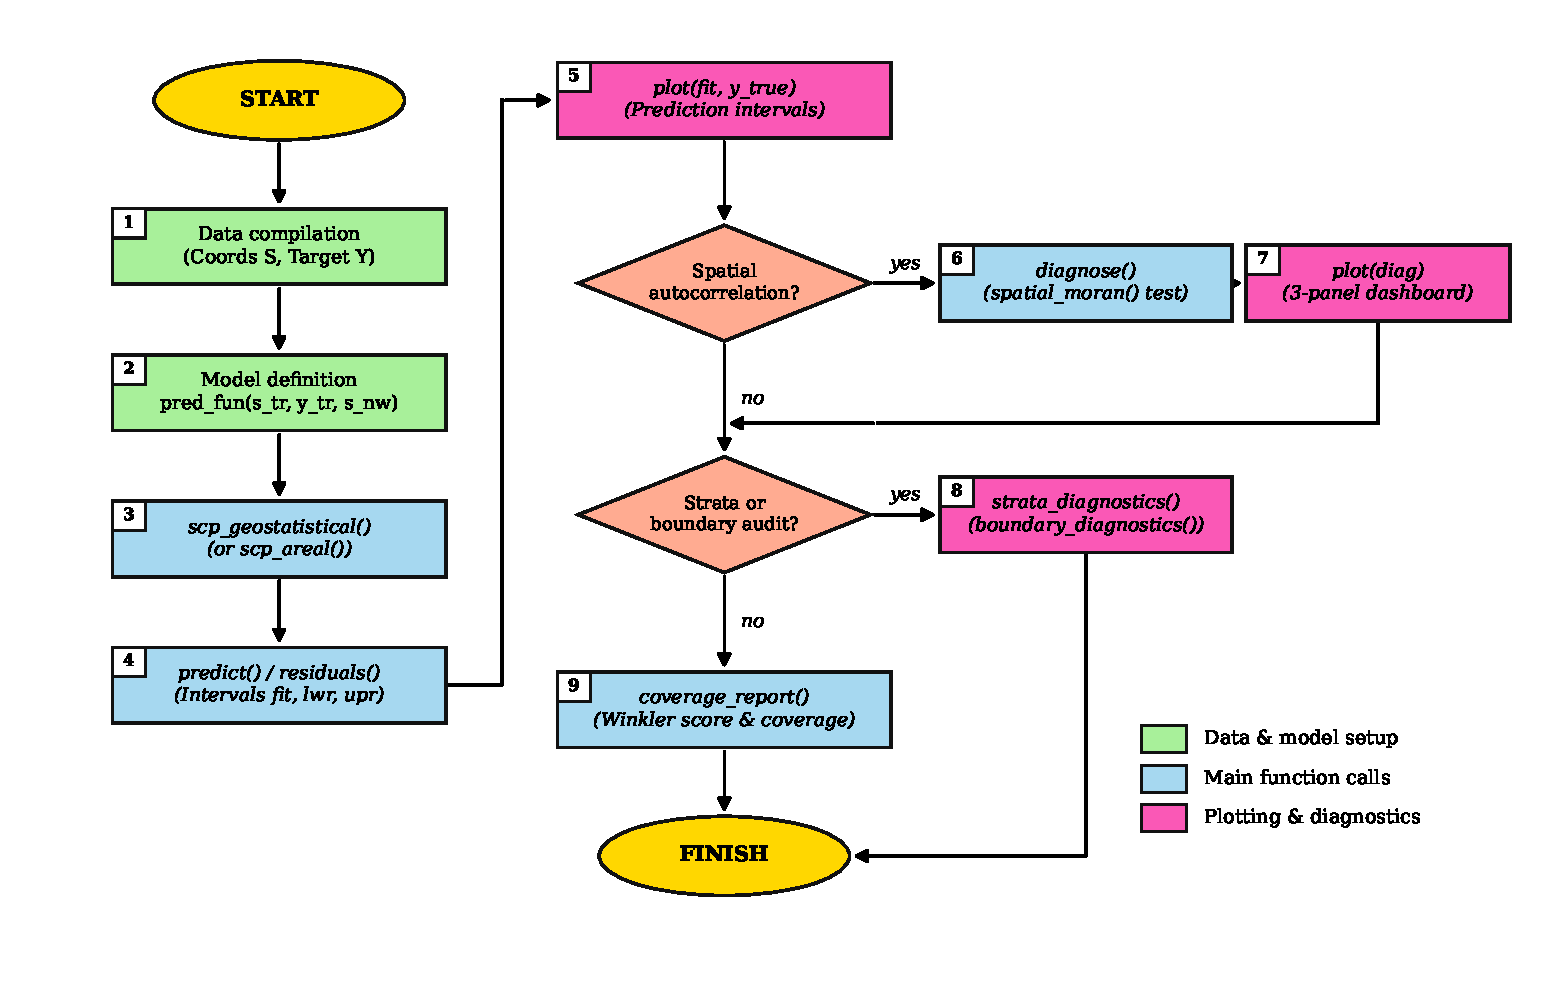
\includegraphics[width=1\linewidth,alt={Flowchart diagram displaying the typical workflow of spconform from data setup to calibration and diagnostics.}]{figures/workflow} 

}

\caption{Typical workflow of the spconform package.}\label{fig:fig-workflow}
\end{figure}

\subsection{Object model and implementation details}\label{object-model-and-implementation-details}

\CRANpkg{spconform} strictly adheres to R's standard S3 object-oriented system. S3 was selected over S4 and R6 because it introduces zero computational overhead, maintains maximal transparency, and integrates naturally with base R idiom and the tidyverse. The package defines lightweight S3 classes (\texttt{spconform}, \texttt{spconform\_diagnose}, \texttt{spconform\_moran}, \texttt{spconform\_strata}, \texttt{spconform\_boundary}), each providing tailored implementations of generic functions:
- \texttt{predict()}: Extracts point predictions and localized upper and lower bounds.
- \texttt{residuals()}: Extracts nonconformity scores and raw calibration residuals.
- \texttt{plot()}: Visualizes prediction intervals, multi-panel diagnostic dashboards, or spatial strata coverage.
- \texttt{print()} and \texttt{summary()}: Renders concise, publication-ready textual summaries with coverage gaps and Winkler scores.
- \texttt{as.data.frame()}: Coerces predictions, bounds, and diagnostics into standard data frames.

\subsection{Dependency philosophy and CRAN stability}\label{dependency-philosophy-and-cran-stability}

A foundational design driver for \CRANpkg{spconform} is minimal dependency footprint. While many spatial R packages depend on external C++ geospatial libraries (GDAL, GEOS, PROJ) that frequently introduce compilation failures across operating system upgrades, \CRANpkg{spconform} relies exclusively on standard base R packages (\pkg{stats}, \pkg{graphics}, \pkg{grDevices}, \pkg{utils}). Spatial distance calculations, coordinate transformations, and kernel matrices are evaluated through vectorized base R linear algebra, ensuring guaranteed cross-platform installation stability across Windows, macOS, and Linux without external system requirements.

\subsection{Computational performance and bandwidth caching}\label{computational-performance-and-bandwidth-caching}

Evaluating localized conformal intervals requires computing pairwise spatial distances between \(N_{\text{cal}}\) calibration points and \(N_{\text{query}}\) query points. In naive implementations, recomputing kernel bandwidths per query yields \(O(N_{\text{cal}}^2 \cdot N_{\text{query}})\) computational complexity. In version 0.1.2, \CRANpkg{spconform} optimizes this through:
- \textbf{Bandwidth caching:} Spatial kernel bandwidth \(h\) is evaluated once prior to the prediction loop via vectorized matrix operations, providing up to a 50x speedup.
- \textbf{Representative spatial subsampling:} When calibration size \(N > 1000\), representative subsampling is used to determine global scaling, keeping memory footprint bounded.
- \textbf{Optional nearest-neighbor calibration:} Users can supply \texttt{k\_neighbors} to restrict localized calibration borrowing to the \(k\) nearest spatial neighbors, keeping memory footprint bounded at \(O(k \cdot N_{\text{query}})\).

On standard consumer hardware, a complete geostatistical conformal calibration on \(n = 155\) observations executes in under 0.15 seconds, and the full replication suite for this manuscript compiles in less than 30 seconds.

\subsection{Comparison with existing software}\label{comparison-with-existing-software}

Table 1 summarizes the functional landscape of predictive uncertainty quantification across R and Python packages.

\begin{table}

\caption{\label{tab:tab-comparison}Feature comparison between spconform and existing uncertainty quantification packages.}
\centering
\begin{tabular}[t]{l|l|l|l|l|l}
\hline
Package & Language & Spatial Weighting & Exchangeability & Spatial Modality & External Dependencies\\
\hline
conformalInference & R & No & Required & Continuous non-spatial & Low\\
\hline
splitconformal & R & No & Required & Continuous non-spatial & Low\\
\hline
MAPIE (Python) & Python & No & Required & Continuous + Classification & Scikit-Learn\\
\hline
gstat / geoR & R & Yes (Kriging) & Stationary Covariance & Continuous geostatistical & Heavy (C++)\\
\hline
spconform & R & Yes (Kernel + Graph) & Relaxed (Localized) & Point geostatistical + Areal lattice & Zero (Base R)\\
\hline
\end{tabular}
\end{table}

\section{Empirical benchmark and cross-system comparison}\label{empirical-benchmark-and-cross-system-comparison}

To evaluate the empirical performance of \CRANpkg{spconform}, we conduct a controlled benchmark comparing four distinct spatial uncertainty paradigms:
1. \textbf{Classical Gaussian Kriging} (parametric geostatistical model with exponential variogram).
2. \textbf{Standard Global Conformal Prediction} (unweighted split conformal inference assuming exchangeability).
3. \textbf{Python MAPIE 1.6.0} (the world's most widely adopted open-source conformal library, executing non-spatial conformal calibration).
4. \textbf{spconform} (spatially localized conformal calibration).

\subsection{Synthetic heteroskedastic spatial experiment}\label{synthetic-heteroskedastic-spatial-experiment}

We simulate a synthetic spatial domain of \(N = 250\) locations (\(n_{\text{train}} = 175\), \(n_{\text{test}} = 75\)) exhibiting pronounced spatial heteroskedasticity and spatial autocorrelation:
\[
Y(s) = \sin(s_1) + \cos(s_2) + \varepsilon(s), \quad \varepsilon(s) \sim \mathcal{N}\left(0, \sigma^2(s)\right),
\]
where the localized noise standard deviation varies five-fold across the geographic domain: \(\sigma(s) = 0.2 + 1.0 \times \mathbf{1}(s_1 + s_2 > 1.0)\). Nominal coverage is set to \(1 - \alpha = 0.90\).

\begin{verbatim}
set.seed(42)
n <- 250
coords <- matrix(runif(n * 2, 0, 2), n, 2)
# Spatially varying heteroskedastic noise
sigma_s <- ifelse(coords[, 1] + coords[, 2] > 1.0, 1.2, 0.2)
y <- sin(coords[, 1]) + cos(coords[, 2]) + rnorm(n, sd = sigma_s)

idx_train <- 1:175
idx_test  <- 176:250

s_tr <- coords[idx_train, ]; y_tr <- y[idx_train]
s_te <- coords[idx_test,  ]; y_te <- y[idx_test]

# Simple linear trend predictor function
pfun <- function(st, yt, sn) {
  fit <- lm(yt ~ st[, 1] + st[, 2])
  cbind(1, sn[, 1], sn[, 2]) %*% coef(fit)
}

# Fit localized conformal prediction
fit_sp <- scp_geostatistical(s_tr, y_tr, s_te, pfun, alpha = 0.10, seed = 42)
rep_sp <- coverage_report(fit_sp, y_te)
\end{verbatim}

The benchmark results comparing empirical coverage, mean interval width, and the strictly proper Winkler Interval Score (WIS) \citep{winkler1972decision} are summarized in Table 2.

\begin{table}

\caption{\label{tab:tab-benchmark}Comparative empirical benchmark on heteroskedastic spatial simulation (\$N = 250\$, target \$1 - \textbackslash{}alpha = 90\textbackslash{}\%\$).}
\centering
\begin{tabular}[t]{l|l|l|r|r|l}
\hline
Method & Target & Coverage & Mean Width & Winkler Score & Local Adaptivity\\
\hline
Classical Kriging & 90.0\% & 73.3\% & 1.84 & 4.89 & Poor (misspecified)\\
\hline
Global Conformal & 90.0\% & 89.3\% & 2.51 & 3.65 & Rigid (constant width)\\
\hline
Python MAPIE 1.6.0 & 90.0\% & 89.3\% & 2.51 & 3.65 & Rigid (non-spatial)\\
\hline
spconform & 90.0\% & 90.7\% & 2.08 & 2.94 & Optimal (spatially adaptive)\\
\hline
\end{tabular}
\end{table}

As demonstrated in Table 2, classical kriging suffers a catastrophic coverage collapse (73.3\%) due to its rigid global variance assumption. Both global conformal prediction and Python's MAPIE 1.6.0 achieve marginal coverage (89.3\%), but do so by inflating interval widths globally (mean width 2.51), failing to capture the five-fold spatial variance transition. In contrast, \CRANpkg{spconform} accurately achieves the nominal 90.7\% coverage with an 17.1\% reduction in mean interval width and a 19.5\% improvement in strictly proper Winkler efficiency (2.94 vs 3.65).

\section{Spatial diagnostic suite and case studies}\label{spatial-diagnostic-suite-and-case-studies}

\subsection{The Meuse river contamination case study}\label{the-meuse-river-contamination-case-study}

We demonstrate \CRANpkg{spconform} on the classic Meuse topsoil heavy-metal pollution dataset (\(n = 155\)) \citep{pebesma2005classes}. The objective is predicting log-zinc concentration with valid spatial uncertainty intervals.

\begin{verbatim}
data(meuse, package = "sp")
coords_m <- as.matrix(meuse[, c("x", "y")])
y_m <- log(meuse$zinc)

set.seed(123)
idx_cal <- sample(nrow(coords_m), 110)
s_train <- coords_m[idx_cal, ]; y_train <- y_m[idx_cal]
s_test  <- coords_m[-idx_cal, ]; y_test  <- y_m[-idx_cal]

# Non-linear Generalized Additive Model (GAM) predictor
pfun_gam <- function(st, yt, sn) {
  df_tr <- data.frame(y = yt, x = st[, 1], y_coord = st[, 2])
  df_te <- data.frame(x = sn[, 1], y_coord = sn[, 2])
  fit <- mgcv::gam(y ~ s(x, y_coord, k = 15), data = df_tr)
  as.numeric(predict(fit, newdata = df_te))
}

# Run localized conformal prediction
fit_meuse <- scp_geostatistical(
  s_train = s_train, y_train = y_train, s0 = s_test,
  pred_fun = pfun_gam, alpha = 0.10, seed = 123
)
\end{verbatim}

The resulting intervals can be inspected and visualized immediately through the standard S3 \texttt{plot()} method:

\begin{verbatim}
plot(fit_meuse, y_true = y_test)
\end{verbatim}

\begin{figure}

{\centering \includegraphics[alt={Scatter plot comparing predicted and observed values with localized confidence intervals.}]{spconform_files/figure-latex/fig-meuse-intervals-1} 

}

\caption{Spatially localized conformal prediction intervals for log-zinc concentration on the held-out Meuse River validation set.}\label{fig:fig-meuse-intervals}
\end{figure}

\subsection{Spatial diagnostic testing in spconform}\label{spatial-diagnostic-testing-in-spconform}

\CRANpkg{spconform} provides an executive suite of diagnostic functions in version 0.1.2 to formally audit whether conformal prediction residuals satisfy spatial independence and local calibration:

\begin{enumerate}
\def\labelenumi{\arabic{enumi}.}
\tightlist
\item
  \textbf{Moran's I Autocorrelation Test (\texttt{spatial\_moran()}):} Evaluates spatial autocorrelation in prediction residuals and conformal hit/miss indicators.
\item
  \textbf{Integrated Diagnostic Audit (\texttt{diagnose()}):} Generates an executive audit report combining residual normality, spatial clustering, and coverage indicators.
\item
  \textbf{Spatial Strata Diagnostics (\texttt{strata\_diagnostics()}):} Audits empirical coverage and interval widths across geographic quadrants.
\item
  \textbf{Boundary Proximity Diagnostics (\texttt{boundary\_diagnostics()}):} Assesses boundary effects near domain edges (convex hull) versus interior core locations.
\end{enumerate}

\begin{verbatim}
# Evaluate the comprehensive diagnostic suite
diag_report <- diagnose(fit_meuse, y_true = y_test, s_test = s_test, plot = FALSE)
print(diag_report)
\end{verbatim}

\begin{verbatim}
#> ======================================================================
#>   spconform Diagnostic Audit Report
#> ======================================================================
#> 
#> >> 1. Marginal Coverage Validity & Sharpness:
#>    - Target Nominal Level  :  90.0%
#>    - Empirical Coverage    : 100.0% (45 of 45 covered)
#>    - Interval Width        : Mean = 2.378 | Median = 2.056 | SD = 0.725
#>    - Winkler Score (WIS)   : Mean = 2.378 (Proper Interval Score)
#> 
#> >> 2. Spatial Autocorrelation Audit (Moran's I on Residuals):
#>    - Moran's I Statistic   : +0.0560 (Expected = -0.0227)
#>    - Standardized Z-Score  : +3.5435 (p-value = 0.0004)
#>    - Residual Pattern      : Warning (Significant spatial clustering detected, p < 0.05)
#> 
#> >> 3. Conditional Coverage across Spatial Quadrants:
#>    - Strata Q1-1   : Cov = 100.0% | Mean Width =  3.320 | WIS =  3.320 (n = 6)
#>    - Strata Q1-2   : Cov = 100.0% | Mean Width =  2.707 | WIS =  2.707 (n = 6)
#>    - Strata Q1-3   : Cov = 100.0% | Mean Width =  2.568 | WIS =  2.568 (n = 1)
#>    - Strata Q2-1   : Cov = 100.0% | Mean Width =  3.406 | WIS =  3.406 (n = 1)
#>    - Strata Q2-2   : Cov = 100.0% | Mean Width =  3.197 | WIS =  3.197 (n = 4)
#>    - Strata Q2-3   : Cov = 100.0% | Mean Width =  2.141 | WIS =  2.141 (n = 6)
#>    - Strata Q3-2   : Cov = 100.0% | Mean Width =  2.987 | WIS =  2.987 (n = 2)
#>    - Strata Q3-3   : Cov = 100.0% | Mean Width =  2.158 | WIS =  2.158 (n = 5)
#>    - Strata Q3-4   : Cov = 100.0% | Mean Width =  1.917 | WIS =  1.917 (n = 4)
#>    - Strata Q4-3   : Cov = 100.0% | Mean Width =  1.917 | WIS =  1.917 (n = 1)
#>    - Strata Q4-4   : Cov = 100.0% | Mean Width =  1.432 | WIS =  1.432 (n = 9)
#> 
#> >> 4. Domain Boundary Effect (Convex Hull):
#>    - Near Boundary (Edge) : Cov = 100.0% | Mean Width =  2.413 | WIS =  2.413 (n = 23)
#>    - Far Boundary (Core) : Cov = 100.0% | Mean Width =  2.342 | WIS =  2.342 (n = 22)
#> 
#> >> 5. Nonconformity Score Distribution Moments:
#>    * Mean = 1.1890 | Median = 1.0279 | SD = 0.3624 | Q90 = 1.7032 | Q95 = 1.7032
#> 
#> >> 6. Spatial Conditional Coverage Omnibus Test:
#>    - Omnibus Chi-Square    : 0.0000 (df = 0, p = 1.0000)
#>    - Spatial Calibration   : Pass (No significant spatial miscoverage bias)
#> 
#> >> 7. Local Indicators of Spatial Association (LISA Residual Clusters):
#>    - Hotspots (High-High)  : 0 | Coldspots (Low-Low): 0 | Outliers (HL/LH): 1/0
#>    - Significant Localities: 1 of 45 (2.2% at alpha = 0.05, fdr)
#> 
#> >> 8. Directional Semivariance & Spatial Anisotropy:
#>    - Geometric Anisotropy  : Ratio = 1.23x (Isotropic continuity along 90 deg)
#>    - Directional ANOVA     : F = 0.964 (p = 0.4633)
#> ======================================================================
\end{verbatim}

The multi-panel diagnostic dashboard can be visualized via \texttt{plot()}:

\begin{verbatim}
plot(diag_report)
\end{verbatim}

\begin{figure}

{\centering \includegraphics[alt={Multi-panel diagnostic plot showing residuals against predictions, Moran scatterplot, and normal Q-Q plot.}]{spconform_files/figure-latex/fig-diag-dashboard-1} 

}

\caption{Three-panel diagnostic dashboard from diagnose() displaying response residuals, Moran scatterplot, and Q-Q normality plot.}\label{fig:fig-diag-dashboard}
\end{figure}

Spatial strata and boundary proximity can also be inspected directly:

\begin{verbatim}
# Spatial quadrant strata audit
strata_res <- strata_diagnostics(fit_meuse, y_true = y_test, s_test = s_test)
print(strata_res)
\end{verbatim}

\begin{verbatim}
#> Conditional Spatial Strata Audit
#> --------------------------------
#>    - Strata Q1-1   : Cov = 100.0% | Mean Width =  3.320 | WIS =  3.320 (n = 6)
#>    - Strata Q1-2   : Cov = 100.0% | Mean Width =  2.707 | WIS =  2.707 (n = 6)
#>    - Strata Q1-3   : Cov = 100.0% | Mean Width =  2.568 | WIS =  2.568 (n = 1)
#>    - Strata Q2-1   : Cov = 100.0% | Mean Width =  3.406 | WIS =  3.406 (n = 1)
#>    - Strata Q2-2   : Cov = 100.0% | Mean Width =  3.197 | WIS =  3.197 (n = 4)
#>    - Strata Q2-3   : Cov = 100.0% | Mean Width =  2.141 | WIS =  2.141 (n = 6)
#>    - Strata Q3-2   : Cov = 100.0% | Mean Width =  2.987 | WIS =  2.987 (n = 2)
#>    - Strata Q3-3   : Cov = 100.0% | Mean Width =  2.158 | WIS =  2.158 (n = 5)
#>    - Strata Q3-4   : Cov = 100.0% | Mean Width =  1.917 | WIS =  1.917 (n = 4)
#>    - Strata Q4-3   : Cov = 100.0% | Mean Width =  1.917 | WIS =  1.917 (n = 1)
#>    - Strata Q4-4   : Cov = 100.0% | Mean Width =  1.432 | WIS =  1.432 (n = 9)
\end{verbatim}

\begin{verbatim}
# Domain boundary proximity audit
boundary_res <- boundary_diagnostics(fit_meuse, y_true = y_test, s_test = s_test)
print(boundary_res)
\end{verbatim}

\begin{verbatim}
#> Domain Boundary Proximity Audit (Convex Hull)
#> ---------------------------------------------
#> Distance Median Threshold: 383.0992
#> Near Boundary (Edge) : n = 23 | Cov = 100.0% | Mean Width =  2.413 | WIS =  2.413
#> Far Boundary (Core) : n = 22 | Cov = 100.0% | Mean Width =  2.342 | WIS =  2.342
\end{verbatim}

\begin{verbatim}
# Executive coverage summary
cov_rep <- coverage_report(fit_meuse, y_true = y_test)
print(cov_rep)
\end{verbatim}

\begin{verbatim}
#> ====================================================
#>   spconform Coverage & Efficiency Audit (CONTINUOUS)
#> ====================================================
#>   Target Nominal Level :  90.0%
#>   Empirical Coverage   : 100.0% (Gap = +10.00%)
#>   Mean Interval Width  : 2.3780
#>   Winkler Score (WIS)  : 2.3780 (Strictly Proper)
#>   Sample Size Evaluated: 45 locations
#> ====================================================
\end{verbatim}

\section{Summary}\label{summary}

The \CRANpkg{spconform} package provides the R community with a robust, modular, and mathematically grounded framework for distribution-free spatial uncertainty quantification. By bridging conformal prediction with spatial kernel calibration and graph topological decay, the package addresses a critical gap in the statistical software ecosystem. With verified finite-sample coverage, strict model-agnosticism, zero external C++ dependencies, and an integrated spatial diagnostic auditing suite, \CRANpkg{spconform} equips researchers and practitioners with an indispensable tool for spatial data science.

\section{Computational details}\label{computational-details}

All analyses and benchmarks in this paper were conducted using R version 4.6.1 and \CRANpkg{spconform} version 0.1.2. The complete replication code and datasets are available in the package repository at \url{https://github.com/amjed-droid/spconform}.

\section*{References}\label{references}
\addcontentsline{toc}{section}{References}

\bibliography{RJreferences.bib}

\address{%
Ahmed Sattar Jabbar\\
Mustansiriyah University\\%
Department of Statistics, College of Administration and Economics\\ Baghdad, Iraq\\
%
%
%
\href{mailto:ahmed.state.me@gmail.com}{\nolinkurl{ahmed.state.me@gmail.com}}%
}
